\section{Reduced Order Observer Design}

\begin{flalign}  \label{observability}
	\vec{{\mathcal O}} = 
	\begin{bmatrix}
		\vec{C} \\
		\vec{C}\vec{A} \\
		\vec{C}\vec{A}^2 \\
		\vec{C}\vec{A}^3 \\
		\vec{C}\vec{A}^4 \\
		\vec{C}\vec{A}^5 \\		
	\end{bmatrix}
	\si{=}
	\begin{bmatrix}
		\ \ 1 & 0 & 0 & 0 & 0 & 0 \ \ \\
		\ \ 0 & 1 & 0 & 0 & 0 & 0 \ \ \\
		\ \ 0 & 0 & 1 & 0 & 0 & 0 \ \ \\
		\ \ 0 & 0 & 0 & 1 & 0 & 0 \ \ \\
		\ \ 0 & 0 & 0 & 0 & 1 & 0 \ \ \\
		\ \ 0 & 0 & 0 & 0 & 0 & 1 \ \ \\
		\ \ 0 & 0 & 0 & 0 & 0 & 0 \ \ \\
		\ \ 0 & 0 & 0 & 0 & 0 & 0 \ \ \\
		\ \ 0 & 0 & 0 & 0 & 0 & 0 \ \ \\
		\ \ 0 & 0 & 0 & 0 & 0 & 0 \ \ \\
		\ \ 0 & 0 & 0 & 0 & 0 & 0 \ \ \\
		\ \ 0 & 0 & 0 & 0 & 0 & 0 \ \ \\
		\ \ 0 & 0 & 0 & 0 & 0 & 0 \ \ \\
		\ \ 0 & 0 & 0 & 0 & 0 & 0 \ \ \\
		\ \ 0 & 0 & 0 & 0 & 0 & 0 \ \ \\
		\ \ 0 & 0 & 0 & 0 & 0 & 0 \ \ \\
		\ \ 0 & 0 & 0 & 0 & 0 & 0 \ \ \\
		\ \ 0 & 0 & 0 & 0 & 0 & 0 \ \ 														
	\end{bmatrix}
\end{flalign}

\begin{figure}[H]
	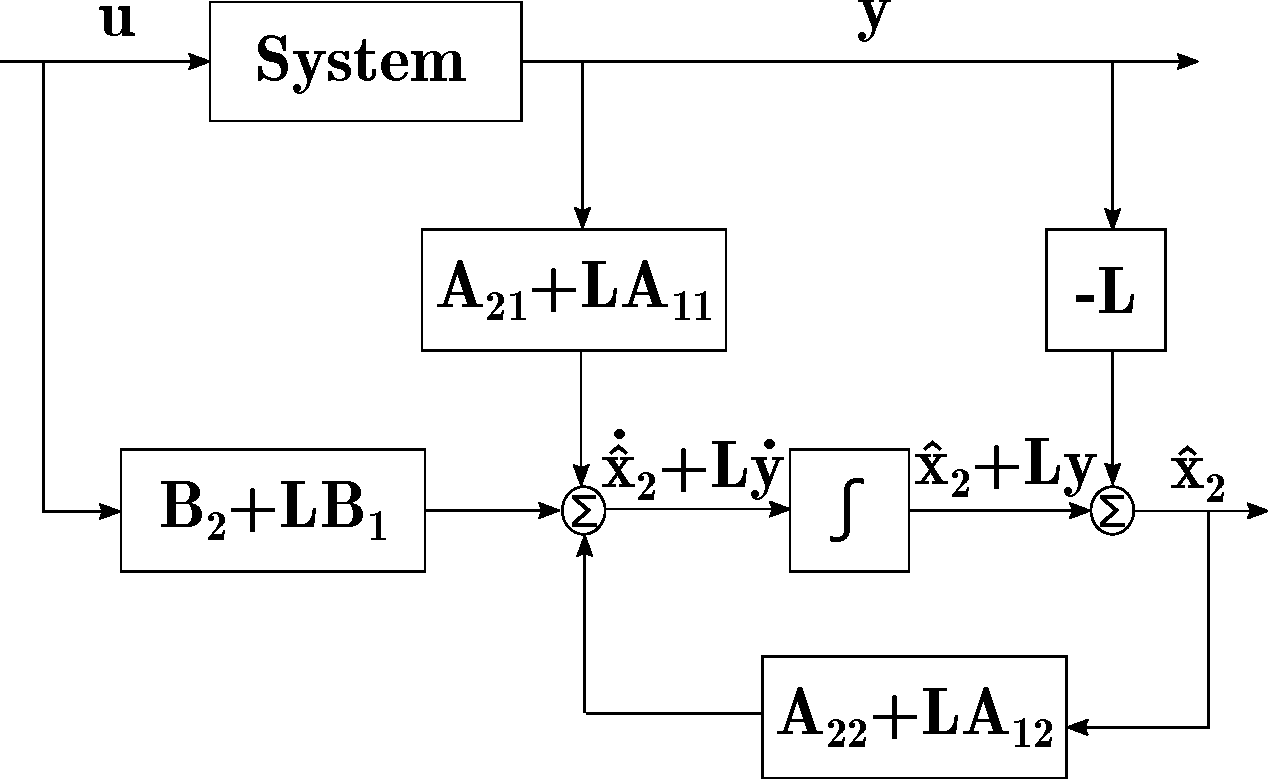
\includegraphics[scale=.35]{figures/observerDiagram}
	\centering
	\captionsetup{justification=centering}
	\captionof{figure}{Diagram . }
	\label{observerDiagram}
\end{figure}


\begin{minipage}{0.15\linewidth}
	\begin{flalign}
	A_{11} = 
	\begin{bmatrix}
		\ 0 & 0 & 0 \ \ \\ 
		\ 0 & 0 & 0 \ \ \\ 
		\ 0 & 0 & 0 \ \ \\
	\end{bmatrix}	\nonumber
	\label{A11}
	\end{flalign}  
\end{minipage}\hfill
\begin{minipage}{0.15\linewidth}
	\begin{flalign}
	A_{12} = 
	\begin{bmatrix}
		\ 1 & 0 & 0 \ \ \\ 
		\ 0 & 1 & 0 \ \ \\ 
		\ 0 & 0 & 1 \ \ \\
	\end{bmatrix}	\nonumber
	\label{A12}
	\end{flalign}
\end{minipage}\hfill
\begin{minipage}{0.15\linewidth}
	\begin{flalign}
	A_{21} = 
	\begin{bmatrix}
		\ 0 & 0 & 0 \ \ \\ 
		\ 0 & 0 & 0 \ \ \\ 
		\ 0 & 0 & 0 \ \ \\
	\end{bmatrix}	\nonumber
	\label{A21}
	\end{flalign}
\end{minipage}\hfill
\begin{minipage}{0.15\linewidth}
	\begin{flalign}
	A_{22} = 
	\begin{bmatrix}
		\ 0 & 0 & 0 & 0 \ \ \\ 
		\ 0 & 0 & 0 & 0 \ \ \\ 
		\ 0 & 0 & 0 & 0 \ \ \\
	\end{bmatrix} 
	\label{A22}
	\end{flalign}
\end{minipage}\hfill


\begin{minipage}{0.5\linewidth}
	\begin{flalign}
	B_1 = 
	\begin{bmatrix}
		\ 0 & 0 & 0 & 0 \ \ \\ 
		\ 0 & 0 & 0 & 0 \ \ \\ 
		\ 0 & 0 & 0 & 0 \ \ \\
	\end{bmatrix}	\nonumber
	\label{B1}
	\end{flalign}
\end{minipage}\hfill
\begin{minipage}{0.5\linewidth}
	\begin{flalign}
	B_2 = 
	\begin{bmatrix}
		0 & \si{-\frac{2 \cdot k_{th} \cdot L \cdot \overline{\omega}_2}{J_x}} & 0 & \si{\frac{2 \cdot k_{th} \cdot L \cdot \overline{\omega}_4}{J_x}} \ \ \ \\ 
		\ \si{\frac{2 \cdot k_{th} \cdot L \cdot \overline{\omega}_1}{J_y}} & 0 & \si{-\frac{2 \cdot k_{th} \cdot L \cdot \overline{\omega}_3}{J_y}} & 0 \ \ \ \\ 
		\frac{2 \cdot k_d \cdot {\overline{\omega}_1}}{J_z} & - \frac{2 \cdot k_d \cdot {\overline{\omega}_2}}{J_z} & \frac{2 \cdot k_d \cdot {\overline{\omega}_3}}{J_z} & - \frac{2 \cdot k_d \cdot {\overline{\omega}_4}}{J_z} \ \ \
	\end{bmatrix}
	\label{B2}
	\end{flalign}
\end{minipage}\hfill


\begin{flalign}
	L = 
	\begin{bmatrix}
	\ -50 & 0 & 0  \ \ \ \\ 
	\ 0 & -60 & 0  \ \ \ \\ 
	\ 0 & 0 & -70  \ \ \  
	\end{bmatrix}
	\label{Lobs}
\end{flalign}


